\section{Equazione di Klein-Gordon}
La motivazione è che l'equazione non relativistica di Schr\"odinger non è adeguata a descrivere i risultati degli esperimenti quando $E>>m_0c^2$. Ricordiamo l'equazione di Schr\"odinger:
\begin{equation}
    -\frac{\hbar^2}{2m} \nabla^2 \psi(\mathbf{r}, t) = i\hbar \frac{\partial}{\partial t} \psi(\mathbf{r}, t)
    \label{eq:schrodinger}
\end{equation}
può essere ricavata partendo dalla relazione:
\begin{equation}
    E=\frac{\mathbf{p}^2}{2m}
\end{equation}
Per ottenerla si danno le seguenti sostituzioni operatoriali:
\begin{equation}
    E\to i\hbar\frac{\partial}{\partial t}\quad \mathbf{p}\to-i\hbar\nabla
\end{equation}
Per giungere ad un'equazione relativistica si può seguire lo stesso metodo utilizzando grandezze e relazioni relativistiche ($c=1$). Infatti il $4-$vettore energia impulso $p^\mu=(E,\mathbf{p})$ con la consueta relazione in notazione covariante:
\begin{equation}
    p^2=p^\nu p_\nu=E^2-\mathbf{p}^2=m^2
\end{equation}
\subsection{Soluzioni dell'equazione di Klein-Gordon}
Per semplicità da ora in poi poniamo $\hbar=c=1$. Sostituendo gli operatori nella relazione energia impulso otteniamo l'equazione di Klein-Gordon
\begin{equation}
    \frac{\partial^2}{\partial t^2}\phi - \nabla^2\phi + m^2\phi = 0
    \label{eq:KG}
\end{equation}
Una soluzione di questa equazione differenziale alle derivate parziali è un'onda piana in cui l'esponente è un prodotto scalare quadridimensionale:
\begin{equation}
    \phi=Ne^{-ip\cdot x}
\end{equation}
dove $p=(E,p)$ e $x=(t,r)$ sono $4-$vettori; $p$ è un parametro. Sostituendo otteniamo:
\begin{equation*}
    -p_0^2\phi+\mathbf{p}^2\phi+m^2\phi=0
\end{equation*}
Perchè l'equazione sia soddisfatta $p$ deve soddisfare la condizione 
\begin{equation*}
    p_0^2=\mathbf{p}^2+m^2
\end{equation*}
Identifichiamo pertanto $p$ con il $4-$impulso della particella e quindi $p_0=E$. La soluzione è caratterizzata da $3$ paramentri indipendenti: $p_x, p_y,p_z$ e notiamo inoltre che:
\begin{equation*}
    E=\pm\sqrt{\mathbf{p}^2+m^2}=\pm E_\mathbf{p} \quad\text{ dove } E_\mathbf{p} \text{ è sempre positivo}
\end{equation*}
Ci sono pertando due soluzioni:
\begin{align*}
    \phi_+ = Ne^{-iE_p t + i\mathbf{p} \cdot \mathbf{r}} \quad \text{soluzione con energia positiva} \\
\phi_- = Ne^{+iE_p t + i\mathbf{p} \cdot \mathbf{r}} \quad \text{soluzione con energia negativa}
\end{align*}
Come nel caso dell'equazione di Schr\"odinger le soluzione trovate sono autofunzioni dell'equazione che hanno uno spettro continuo e quindi non sono normalizzabili. Le soluzioni per problemi fisici si ottengono costruendo pacchetti d'onda:
\begin{equation}
    \phi(\mathbf{r}, t)=\int_{-\infty}^{+\infty} \frac{d^3 \mathbf{k}}{(2 \pi)^3 \sqrt{2 E_{\mathbf{k}}}}\left[a(\mathbf{k}) e^{-i E_{\mathbf{k}} t+i \mathbf{k} \cdot \mathbf{r}}+b(\mathbf{k}) e^{+i E_{\mathbf{k}} t+i \mathbf{k} \cdot \mathbf{r}}\right]
\end{equation}
Sfruttando la simmetria dell'integrazione in $\mathbf{k}$ si può cambiare segno della parte spaziale dell'esponenziale del secondo termine dell'integrale. Dobbiamo però ricordare che $b(\mathbf{k})$ è una funzione arbitraria (anche $a(\mathbf{k})$) e quindi possiamo chiamare ancora $b(\mathbf{k})$ la funzione $b(-\mathbf{k})$:
\begin{equation}
    \phi(\mathbf{r}, t)=\int_{-\infty}^{+\infty} \frac{d^3 \mathbf{k}}{(2 \pi)^3 \sqrt{2 E_{\mathbf{k}}}}\left[a(\mathbf{k}) e^{-i E_{\mathbf{k}} t+i \mathbf{k} \cdot \mathbf{r}}+b(\mathbf{k}) e^{+i E_{\mathbf{k}} t\textcolor{red}{-}i \mathbf{k} \cdot \mathbf{r}}\right]
\end{equation}
Introduciamo il prodotto scalare quadridimensionale: $k\cdot x=E_\mathbf{k}t-\mathbf{k}\cdot\mathbf{r}$
\begin{equation}
    \phi(\mathbf{r}, t)=\int_{-\infty}^{+\infty} \frac{d^3 \mathbf{k}}{(2 \pi)^3 \sqrt{2 E_{\mathbf{k}}}}\left[a(\mathbf{k}) e^{-ik\cdot x}+b(\mathbf{k}) e^{+i k\cdot x}\right]
\end{equation}
\section{Corrente di Probabilità}
Abbiamo visto che ci sono soluzioni con energia positiva e negativa ma per ora non abbiamo visto nessun tipo di "inconsistenza". Per questo calcoliamo le correnti di probabilità. Nella meccanica quantistica non relativistica anche lì si arriva a delle autofunzioni dell'operatore di Schr\"odinger che appartengono allo spettro continuo e si costruiscono dei pacchetti. Quello che si dimostra, visto che l'operatore differenziale laplaciano è hermitiano allora esistono un sistema completo di autofunzioni. Anche qui ci sono teoremi analoghi. Quindi in questa equazione dal punto di vista matematico ci dice che ogni funzione può essere sviluppata con questo sistema di autofunzioni completo dell'operatore di Klein-Gordon. Questo teorema di completezza è fondamentale e quindi questo termine di energia negativa non si può semplicemente cancellare.
\subsection{Schr\"odinger}
Consideriamo l'equazione di Schr\"odinger e la sua complessa coniugata
$$
i \frac{\partial \psi}{\partial t}+\frac{1}{2 m} \nabla^2 \psi=0 \quad-i \frac{\partial \psi^*}{\partial t}+\frac{1}{2 m} \nabla^2 \psi^*=0
$$
Moltiplichiamo a sinistra rispettivamente per $\psi^*$ e $\psi$
$$
i \psi^* \frac{\partial \psi}{\partial t}+\frac{1}{2 m} \psi^* \nabla^2 \psi=0 \quad-i \psi \frac{\partial \psi^*}{\partial t}+\frac{1}{2 m} \psi \nabla^2 \psi^*=0
$$
Sottraiamo le due equazioni
$$
i \psi^* \frac{\partial \psi}{\partial t}+\frac{1}{2 m} \psi^* \nabla^2 \psi+i \psi \frac{\partial \psi^*}{\partial t}-\frac{1}{2 m} \psi \nabla^2 \psi^*=0
$$
Elaborando
$$
i \frac{\partial}{\partial t}\left(\psi^* \psi\right)+\frac{1}{2 m} \nabla\left(\psi^* \nabla \psi-\psi \nabla \psi^*\right)=0 \quad \frac{\partial}{\partial t}|\psi|^2+\frac{-i}{2 m} \nabla\left(\psi^* \nabla \psi-\psi \nabla \psi^*\right)=0
$$
Definendo
$$
\rho=|\psi|^2 \quad \mathbf{J}=\frac{-i}{2 m}\left[\psi^* \boldsymbol{\nabla} \psi-\psi \boldsymbol{\nabla} \psi^*\right]
$$
Otteniamo
$$
\frac{\partial}{\partial t} \rho+\nabla \cdot \mathbf{J}=0
$$
equazione di continuità per la probabilità. Questo ci dice che la probabilità nella meccanica quantistica è una grandezza che si conserva localmente. Una volta che ho definito una funzione d'onda so che in una certa regione nello spazio ho una probabilità. Se questa probabilità cambia nel tempo lo deve fare in modo che ci sia una corrente di probabilità che porta via probabilità da un punto nello spazio analogamente alla densità di carica in elettrodinamica. Deriva dalla natura hermitiana dell'equazione di Schr\"odinger. Nel caso particolare delle soluzioni:
\begin{equation*}
    \psi=Ne^{-i\left(\frac{\mathbf{p}^2}{2m}t-\mathbf{p}\cdot\mathbf{x}\right)}
\end{equation*}
Otteniamo
\begin{equation*}
    \rho=|N|^2 \qquad \mathbf{J}=\frac{-i}{2m}|N|^2[i\mathbf{p}+i\mathbf{p}]=|N|^2\frac{\mathbf{p}}{m}
\end{equation*}
\begin{equation*}
    \mathbf{J}=\rho\frac{\mathbf{p}}{m}=\rho\mathbf{v}
\end{equation*}
\subsection{Klein-Gordon}
Dobbiamo adesso verificare se le soluzione dell'equazione di Klein-Gordon consentono lo stesso tipo di interpretazione che si era sviluppata per le soluzione dell'equazione di Schr\"odinger. Procedendo in modo del tutto analogo a quanto fatto per l'equazione di Schr\"odinger:
$$
\frac{\partial^2}{\partial t^2} \phi-\nabla^2 \phi+m^2 \phi=0 \quad \frac{\partial^2}{\partial t^2} \phi^*-\nabla^2 \phi^*+m^2 \phi^*=0
$$
Moltiplichiamo a sinistra per $\phi^*$ e $\phi$
$$
\phi^* \frac{\partial^2}{\partial t^2} \phi-\phi^* \nabla^2 \phi+m^2 \phi^* \phi=0 \quad \phi \frac{\partial^2}{\partial t^2} \phi^*-\phi \nabla^2 \phi^*+m^2 \phi^* \phi=0
$$
Sottraiamo
$$
\phi^* \frac{\partial^2}{\partial t^2} \phi-\phi^* \nabla^2 \phi-\phi \frac{\partial^2}{\partial t^2} \phi^*+\phi \nabla^2 \phi^*=0
$$

Si giunge alla definizione di densità di probabilità
$$
\rho=i\left(\phi^* \frac{\partial}{\partial t} \phi-\phi \frac{\partial}{\partial t} \phi^*\right)
$$
Definizione di densità di corrente di probabilità
$$
\mathbf{J}=-i\left(\phi^*\nabla\phi-\phi\nabla\phi^*\right)
$$
Equazione di Continuità
$$
\frac{\partial}{\partial t} \rho+\nabla \cdot \mathbf{J}=0
$$
Ancora una volta, specializzando alle soluzione di onda piana: $\phi=Ne^{-ip\cdot x}$ calcoliamo la densità di probabilità. Questa definizione porta alla prima inconsistenza dell'equazione di Klein-Gordon:
\begin{itemize}
    \item Per le soluzioni a energia positiva (ricordiamo che $E_\mathbf{p}>0$ sempre) $$ \phi_+ = Ne^{-iE_p t + i\mathbf{p} \cdot \mathbf{r}} \qquad \rho=|N|^2i(-iE_\mathbf{p}-iE_\mathbf{p})=2|N|^2E_\mathbf{p}>0$$
    \item Per le soluzioni a energia negativa
    $$ \phi_- = Ne^{+iE_p t + i\mathbf{p} \cdot \mathbf{r}} \qquad \rho=|N|^2i(iE_\mathbf{p}+iE_\mathbf{p})=-2|N|^2E_\mathbf{p}<0$$
\end{itemize}
Pertanto le soluzione a energia negativa portano ad una probabilità negativa. Questo è privo di qualsiasi senso fisico. Le soluzioni non hanno quindi un'interpretazione fisica ben definita. La prima tentazione sarebbe quella di buttare via le soluzioni ad energia negativa ma questo è impossibile in quando per avere la completezza delle nostre soluzione dobbiamo avere anche quelle con energia negativa. Notiamo che matematicamente la probabilità negativa è una conseguenza del fatto che l'equazione di Klein-Gordon è di secondo grado nel tempo. Torneremo in seguito su questo problema, al momento irrisolto. 
\section{Invarianza relativistica dell'equazione di Klein-Gordon}
Un importante requisito delle equazioni relativistiche è la loro invarianza relativistica. Formalmente le equazioni relativistiche devono avere la stessa forma in tutti i sistemi di riferimento inerziali. Considerndo l'equazione di Klein-Gordon ($\partial_\mu\equiv\partial/\partial x^\mu$)
\begin{equation}
    \left(\frac{\partial^2}{\partial t^2} - \nabla^2 + m^2\right)\phi = 0 \qquad \left(\partial^\mu\partial_\mu+m^2\right)\phi=0
\end{equation}
Consideriamo un passaggio da un sistema interziale $\mathbf{K}$ ad un sistema $\mathbf{K}'$ tramite una trasformazione di Lorentz $\Lambda$. Come si trasformano gli operatori di derivazione $\partial_\mu$ e $\partial^\mu$? come si trasforma la funzione $\phi(x)$? La massa $m$ è invariante (infatti è uno scalare in una trasformazione di Lorentz). Approfondiamo innanzitutto le proprietà delle trasformazioni di Lorentz.
\subsection{Trasformazioni di Lorentz}
In una trasformazione di Lorentz (ad esempio un boost lungo l'asse $x$) le componenti del $4-$vettore tempo-posizione si trasformano secondo la legge:
\begin{figure}[h!]
    \centering
    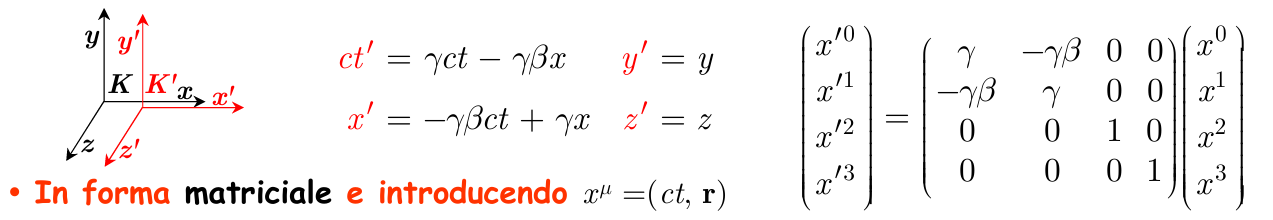
\includegraphics[width=1.1\textwidth]{Lezioni/Lezione 1/KK.png}
    \label{fig:KK}
\end{figure}
Conviene esprimere il prodotto matriciale in forma tensoriale:
\begin{equation*}
    x'^\mu=\Lambda^\mu_{\,\,\nu}x^\nu \quad \text{ sottointesa la somma dell'indice contratto }\nu
\end{equation*}
Notare le posizione degli indici $\mu$ e $\nu$ e i segni degli elementi della matriche che sorrisponde a questa disposizione degli indici:
\begin{equation*}
    g_{\mu\alpha}g^{\alpha\nu}=g_\mu^{\,\,\nu}=\delta_\mu^{\,\,\nu}
\end{equation*}
Altre forme della matrice:
\begin{figure}[h!]
    \centering
    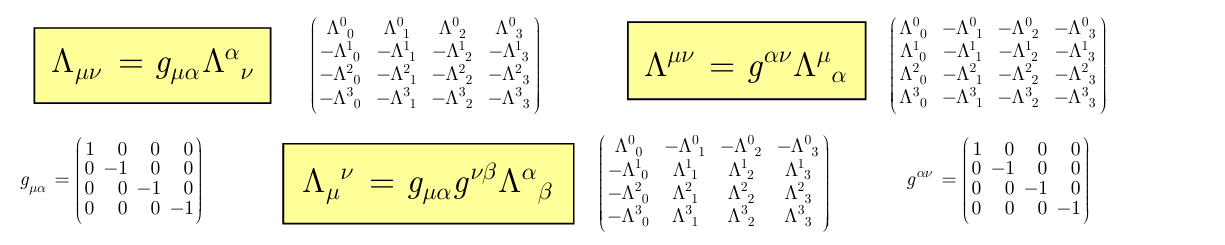
\includegraphics[width=1.1\textwidth]{Lezioni/Lezione 1/Ss.png}
    \label{fig:Ss}
\end{figure}
La proprietà che caratterizza una trasformazione di Lorentz è l'invarianza del prodotto scalare:
\begin{equation*}
    x'\cdot y'=x'^\mu y'_\mu=x\cdot y=x^\mu y_\mu
\end{equation*}
Introducendo le coordinate nel sistema $\mathbf{K}'$
\begin{equation*}
    x'^\mu=\Lambda^\mu_{\,\,\nu}x^\nu \qquad y'^\mu=\Lambda^\mu_{\,\,\nu}y^\nu
\end{equation*}
\begin{equation*}
    x'^\mu y'_\mu = g_{\mu\nu} x'^\mu y'^\nu = g_{\mu\nu} \Lambda^\mu_{\,\,\alpha} x^\alpha \Lambda^\nu_{\,\,\beta} y^\beta = (g_{\mu\nu} \Lambda^\mu_{\,\,\alpha} \Lambda^\nu_{\,\,\beta}) x^\alpha y^\beta = g_{\alpha\beta} x^\alpha y^\beta
\end{equation*}
In conclusione:
\begin{equation*}
    g_{\mu\nu}\Lambda^\mu_{\,\,\alpha}\Lambda^\nu_{\,\,\beta}=g_{\alpha\beta}
\end{equation*}
In forma matriciale:
\begin{equation*}
    \Lambda^TG\Lambda=G \quad \text{ in quanto } \quad \Lambda^{\textcolor{red}{\mu}}_{\,\,\alpha}g_{\textcolor{red}{\mu}\textcolor{blue}{\nu}}\Lambda^{\textcolor{blue}{\nu}}_{\,\,\beta}=g_{\alpha\beta}
\end{equation*}
\begin{figure}[h!]
    \centering
    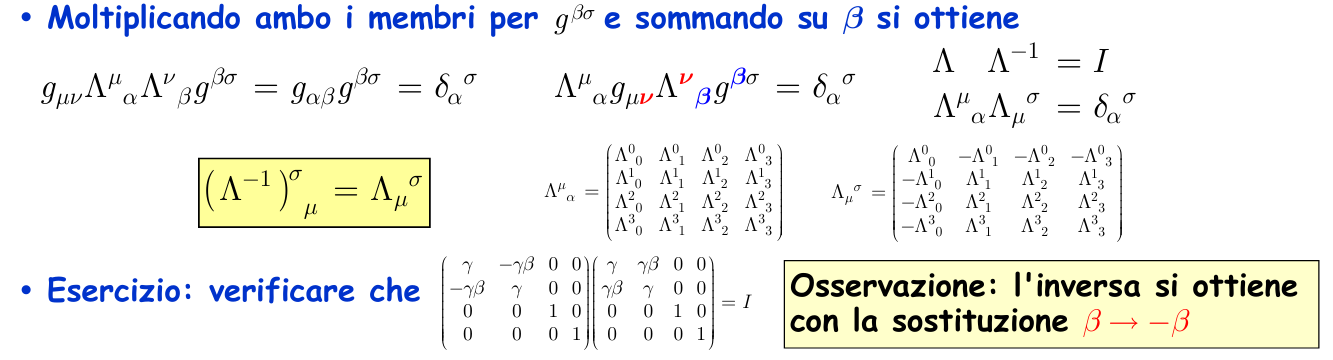
\includegraphics[width=1\textwidth]{Lezioni/Lezione 1/dd.png}
    \label{fig:dd}
\end{figure}
\subsection{Operatore di derivazione}
Verifichiamo le proprietà di trasformazione del $4-$vettore $\partial_\mu\equiv\partial/\partial x^{\mu}$:
si ha ovviamente che:
\begin{equation*}   
    \frac{\partial}{\partial x'^\mu} = \frac{\partial x^\alpha}{\partial x'^\mu} \frac{\partial}{\partial x^\alpha}
\end{equation*}
Ricaviamo l'espressione di $x$ in funzione di $x'$:
\begin{equation*}
    x'^\mu = \Lambda^\mu_{\,\,\nu} x^\nu \qquad \Lambda_\mu^{\,\,\alpha} x'^\mu = \Lambda_\mu^{\,\,\alpha} \Lambda^\mu_{\,\,\nu} x^\nu \qquad \Lambda_\mu^{\,\,\alpha} x'^\mu = \delta^\alpha_{\,\,\nu} x^\nu = x^\alpha
\end{equation*}

\begin{equation*}
    x^\alpha = \Lambda_\mu^{\,\,\alpha} x'^\mu
\end{equation*}
Pertanto
\begin{equation*}
    \frac{\partial x^\alpha}{\partial x'^\mu} = \Lambda_\mu^{\,\,\alpha} \qquad \displaystyle \frac{\partial}{\partial x'^\mu} = \Lambda_\mu^{\,\,\alpha} \frac{\partial}{\partial x^\alpha}
\end{equation*}
Le componenti $\partial/\partial x^\mu$ si trasformano come $x_\mu$ vale a dire in modo covariante:
\begin{equation*}
    \partial_\mu \equiv \frac{\partial}{\partial x^\mu} = \left(\frac{1}{c}\frac{\partial}{\partial t}, \frac{\partial}{\partial x}, \frac{\partial}{\partial y}, \frac{\partial}{\partial z}\right) = \left(\frac{1}{c}\frac{\partial}{\partial t}, \nabla\right)
\end{equation*}
Analogamente abbiamo le componenti controvarianti:
\begin{equation*}
    \frac{\partial}{\partial x_\mu} \equiv \partial^\mu = \left(\frac{1}{c}\frac{\partial}{\partial t}, -\nabla\right) \qquad \displaystyle \frac{\partial}{\partial x'_\mu} = \Lambda^\alpha_{\,\,\mu} \frac{\partial}{\partial x_\alpha}
\end{equation*}
\subsection{Operatore di D'Alambert}
Introduciamo l'operatore di D'Alambert (o d'Alambertiano)
\begin{equation}
    \Box\equiv\frac{\partial}{\partial x^\mu}\frac{\partial}{\partial x_\mu}\equiv\partial^\mu\partial_\mu
\end{equation}
Questo è un operatore scalare. Infatti è il prodotto scalare di un $4-$vettore con se stesso e ha la stessa forma in tutti i sistemi di riferimento. In forma esplicita ($c=1$)
\begin{equation}
    \partial^\mu\partial_\mu=\frac{\partial^2}{\partial t^2}-\nabla^2
\end{equation}
Per finire scriviamo la corrente di probabilità dell'equazione di Klein-Gordon in forma covariante
\begin{equation}
    j^\mu=i\left[\phi^*\partial^\mu\phi-\left(\partial^\mu\phi^*\right)\phi\right]\qquad \partial_\mu j^\mu=0
\end{equation}
\subsection{L'invarianza relativistica dell'equazione di KG}
A questo punto abbiamo tuti gli ingredienti per discutere l'invarianza relativistica dell'equazione di Klein-Gordon. La funzione $\phi(x)$ soddisfa l'equazione di Klein-Gordon nel sistema inerziale $\mathbf{K}$
\begin{equation}
    \left(\partial^\mu\partial_\mu+m^2\right)\phi(x)=0
\end{equation}
Alla funzione $\phi(x)$ corrisponderà una funzione $\phi'(x')$ nel sistema $\mathbf{K}'$. Se richiediamo che l'equazione di Klein-Gordon sia invariante per trasformazioni di Lorentz dovrà valere:
\begin{equation}
        \left(\partial'^\mu\partial'_\mu+m^2\right)\phi'(x')=0
\end{equation}
Dal momento che $\partial^\mu\partial_\mu$ è invariante e che $m$ è invariante è necessario che:
\begin{equation*}
    \phi(x)=\phi'(x')\quad \text{ con } \quad x'^\mu = \Lambda^\mu_{\,\,\nu} x^\nu
\end{equation*}
La condizione sopra riportata definisce la funzione scalare $\phi'(x')$. In punti $x$ e $x'$ rappresentano lo stesso punto nello spazio-tempo visto in due differenti sistemi inerziali. La forma funzionale di $\phi'$ può essere differente da $phi$. Esempio:
\begin{equation*}
    \phi(x)=e^{-ikx} \qquad \phi'(x')=e^{-ik'x'}
\end{equation*}
\section{Eq. di Klein-Gordon: Interpretazione}
Abbiamo visto che le soluzioni con energia negativa portano ad una probabilità negativa che non ha senso fisico. Dirac riuscì a risolvere il problema del segno della probabilità impostando un'equazione del primo ordine. Potremmo tentare di utilizzare l'equazione di Klein-Gordon utilizzando solo le soluzione con energia positiva. Ci sono comunque inconsistenze ad esempio il Paradosso di Klein che è comunque presente anche nell'equazione di Dirac. Studiamo l'interazione di una particella con un campo elettrostatico. L'interazione elettromagnetica viene introdotta tramite la sostituzione:
\begin{equation*}
    \partial^\mu\to\partial^\mu+iqA^\mu
\end{equation*}
\begin{itemize}
    \item Per la componente temporale: $E\to i\frac{\partial}{\partial t}$ $\quad E_t=E-qA^0\equiv E-U$
    \item Per la componente spaziale $\mathbf{p}\to-i\nabla$ $\quad\mathbf{P}=\mathbf{p}-q\mathbf{A}$
\end{itemize}
\section{Il Paradosso di Klein}
Poniamo $\Psi_{E}(z, t)=\psi(z)e^{-iEt}$ (soluzione con $E>0$) e consideriamo l'equazione di Klein-Gordon in presenza di un potenziale a barriera $U=qA^0$ ($A^\mu=\left(A^0,\mathbf{0}\right)$). L'equazione diventa:
\begin{equation*}
(E-U)^{2}\psi(z)=-\frac{d^{2}\psi(z)}{dz^{2}}+m^{2}\psi(z)
\label{eq:KG_potential}
\end{equation*}
\begin{figure}
    \centering
    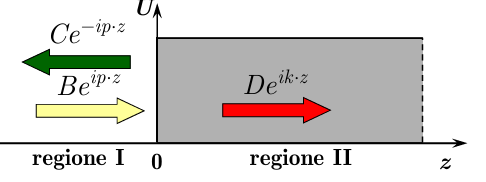
\includegraphics[width=0.8\textwidth]{Lezioni/Lezione 1/tt.png}
    \label{fig:tt}
\end{figure}
Cerchiamo soluzioni stazionarie. La funzione d'onda consiste di due parti:
\begin{itemize}
    \item A sinistra (regione I, $U=0$): un'onda incidente e una riflessa.
    \begin{equation*}
    \psi_{I}(z)=Be^{ip\cdot z}+Ce^{-ip\cdot z}
    \end{equation*}
   
    \item A destra (regione II, $U \ne 0$): un'onda trasmessa.
    \begin{equation*}
    \psi_{II}(z)=De^{ik\cdot z}
    \end{equation*}
\end{itemize}
Sostituendo nell'equazione \ref{eq:KG_potential}, otteniamo le relazioni di dispersione nelle due regioni:
\begin{equation*}
E^{2}=p^{2}+m^{2} \quad \text{} \qquad (E-U)^{2}=k^{2}+m^{2} \quad \text{}
\end{equation*}
Da cui si ricavano $p$ e $k$:
\begin{equation*}
p=\pm\sqrt{E^{2}-m^{2}} \quad \text{} \qquad k=\pm\sqrt{(E-U)^{2}-m^{2}} \quad \text{}
\end{equation*}
Deve essere $p>0$ (B viaggia da sx a dx) mentre il segno di $k$ deve essere determinato.
Imponendo la continuità di $\psi$ e $d\psi/dz$ in $z=0$ si ottiene il sistema:
\begin{equation*}
\begin{cases}B+C=D\\ ipB-ipC=ikD\end{cases}
\end{equation*}
Risolvendo in funzione di $B$ (ampieza incidente) troviamo $C$ (ampiezza riflessa) e $D$ (ampiezza trasmessa):
\begin{equation*}
C=\frac{p-k}{p+k}B \qquad D=\frac{2p}{p+k}B
\end{equation*}
Riepilogando:
\begin{equation*}
    \Psi_E(z,t) = \psi(z) e^{-iEt}
\end{equation*}
\begin{equation*}
    \psi_I(z) = Be^{ip z} + Ce^{-ip z} \qquad \qquad E^2 = p^2 + m^2
\end{equation*}
\begin{equation*}
    \psi_{II}(z) = D e^{ik z} \qquad \qquad (E - U)^2 = k^2 + m^2
\end{equation*}
Le soluzioni normalizzabili si ottengono formando dei pacchetti d'onda:
\begin{equation*}
        \Phi(z,t) = \int g(\xi) \Psi_E(z,t) d\xi = \int g(\xi) \psi(z) e^{-iE(\xi)t} d\xi
        \qquad
        \begin{array}{l}
            \text{regione I} \to \xi = p \\
            \text{regione II} \to \xi = k
        \end{array}
\end{equation*}
Come è noto, nel caso di pacchetti con una definizione del momento molto netta ($g(\xi)$ molto stretta) il pacchetto viaggia senza deformarsi con velocità di gruppo:
\begin{equation*}
    v_g=\frac{\partial E}{\partial \xi}
\end{equation*}
Calcoliamo adesso la corrente di probabilità $j=\frac{1}{2im}(\Psi^{*}\frac{\partial}{\partial z}\Psi-\Psi\frac{\partial}{\partial z}\Psi^{*})$ e la densità di probabilità $\rho=\frac{E-U}{m}|\Psi|^{2}$. Nelle due regioni otteniamo:
\begin{equation*}
j_{I}=\frac{p}{m}(|B|^{2}-|C|^{2}) \quad \text{} \qquad j_{II}= \begin{cases} \frac{k}{m}|D|^{2} & \text{k reale} \\ 0 & \text{k immaginario} \end{cases}
\end{equation*}

\begin{equation*}
\rho_{I}=\frac{E}{m}|\psi_{I}|^{2} \quad \text{} \qquad \rho_{II}=\frac{E-U}{m}|\psi_{II}|^{2} \quad \text{}
\end{equation*}
Definiamo i flussi incidente $j_i=\frac{p}{m}|B|^{2}$, riflesso $j_r=\frac{p}{m}|C|^{2}$ e trasmesso $j_t=j_{II}$. I coefficienti di riflessione $\mathcal{R}$ e trasmissione $\mathcal{T}$ sono:
\begin{equation*}
\mathcal{R}=\frac{j_{r}}{j_{i}}=\left|\frac{C}{B}\right|^{2}=\left|\frac{p-k}{p+k}\right|^{2}
\end{equation*}

\begin{equation*}
\mathcal{T}=\frac{j_{t}}{j_{i}}=\frac{k}{p}\left|\frac{D}{B}\right|^{2}=\frac{k}{p}\left|\frac{2p}{p+k}\right|^{2} \quad (\text{per k reale})
\end{equation*}
Interpretiamo questi risultati al variare di $U$ per un'energia $E$ fissata ($E>m$):
\begin{itemize}
    \item \textbf{Caso 1: $0 < U < E-m$}
    $k$ è reale. Per avere un'onda che viaggia verso destra ($v_g > 0$), scegliamo $k>0$. La velocità di gruppo $v_{g}=\frac{\partial E}{\partial k}=\frac{k}{E-U}$ è positiva e la densità $\rho_{II}=\frac{E-U}{m}|\psi_{II}|^{2}$ è positiva. Si ha un urto analogo alla Meccanica Quantistica non relativistica.
    
    \item \textbf{Caso 2: $E-m < U < E+m$}
    $k=i\kappa$ diventa immaginario. Non si ha propagazione di onda nella regione II. La densità $\rho_{II}$ decresce esponenzialmente e può essere negativa (poiché $E-U < 0$). Si ha riflessione totale:
    \begin{equation*}
    \mathcal{R}=\left|\frac{p-i\kappa}{p+i\kappa}\right|^{2}=1 \qquad \mathcal{T}=0
    \end{equation*}
   
    
    \item \textbf{Caso 3: $U > E+m$}
    $k$ è di nuovo reale. Questo è proibito in M.Q. non relativistica.
    La densità di probabilità è negativa: $\rho_{II}=\frac{E-U}{m}|\psi_{II}|^{2} < 0$.
    La velocità di gruppo è $v_{g}=k/(E-U)$. Dato che $E-U < 0$, per mantenere un'onda che viaggia verso destra ($v_g > 0$) dobbiamo scegliere $k < 0$.
    Con $k<0$, i coefficienti diventano paradossali:
    \begin{equation*}
    \mathcal{R}=\left|\frac{p-k}{p+k}\right|^{2}=\left(\frac{p+|k|}{p-|k|}\right)^{2} > 1
    \end{equation*}
   
    \begin{equation*}
    \mathcal{T}=\frac{j_{t}}{j_{i}}=\frac{k}{p}\left|\frac{2p}{p+k}\right|^{2}=-\frac{4p|k|}{(p-|k|)^{2}} < 0
    \end{equation*}
   
    L'onda riflessa è più intensa di quella incidente ($\mathcal{R}>1$) e la trasmissione è negativa ($\mathcal{T}<0$). Questo risultato, fisicamente assurdo nell'interpretazione a singola particella, è noto come \textbf{Paradosso di Klein}.
\end{itemize}

\section{Meccanica Quantistica e Relatività}
Il principio di indeterminazione di Heisenberg lega l'incertezza sulla posizione $q$ e sulla quantità di moto $p$:
\begin{equation}
\Delta q\Delta p\ge\hbar/2
\end{equation}

La Relatività Ristretta richiede che tempo ed energia siano trattati come le componenti spaziali, formando dei quadrivettori:
\begin{equation*}
x^{\mu}=(ct,x,y,z) \quad \text{} \qquad p^{\mu}=(E,p_{x},p_{y},p_{z}) \quad \text{}
\end{equation*}
La covarianza relativistica impone pertanto un'ulteriore relazione di indeterminazione:
\begin{equation}
\Delta E\Delta t\ge\hbar/2
\end{equation}

Il significato di questa relazione è che l'energia di un sistema può non essere esattamente definita se misurata in intervalli di tempo $\Delta t$ troppo brevi.
L'equivalenza tra massa ed energia $E=mc^2$ implica che l'indeterminazione sull'energia $\Delta E$ possa manifestarsi con l'apparizione di nuove particelle, seppur per tempi brevi (stati virtuali).
Di conseguenza:
\begin{itemize}
    \item La teoria non ha più un numero costante di particelle.
    \item Il paradosso di Klein mostra che il tentativo di "localizzare" una particella con una barriera di potenziale porta a contraddizioni (creazione di coppie).
    \item Il significato di una funzione d'onda delle coordinate va rivisto.
    \item Lo spazio $\mathbf{r}=(x,y,z)$ e il tempo $t$ devono essere trattati allo stesso modo: diventano parametri e non variabili dinamiche.
\end{itemize}
